\documentclass[12pt]{article}

% --- Packages ---
\usepackage[utf8]{inputenc}
\usepackage[T1]{fontenc}
\usepackage[french]{babel}
\usepackage{amsmath, amssymb}
\usepackage{geometry}
% \usepackage[draft]{graphicx}
\usepackage{tikz}
\usepackage[most]{tcolorbox}
\usepackage{multicol}
\usepackage{lmodern}
\usepackage{pgfplots}
\pgfplotsset{compat=1.18}
\usepackage{mdframed}
\usepackage{array}
\usepackage[thinlines]{easytable}
\usepackage{tkz-tab}
\usepackage{bm}
\usepackage{xcolor}
\usepackage{sectsty}
\usepackage[utf8]{inputenc}
\usepackage[T1]{fontenc}
\usepackage[inline]{enumitem}
\usepackage[dvipsnames]{xcolor}
\usepackage{multido}
% --- Page ---
\geometry{margin=2cm}

% Footer
\usepackage{fancyhdr}
\pagestyle{fancy}
\cfoot{\thepage}
\rfoot{\textit{G.M.}}
\renewcommand{\headrulewidth}{0pt}
\renewcommand{\footrulewidth}{0pt}

% Pour les normes : 
\newcommand*{\norme}[1]{\left\lVert\overrightarrow{#1}\right\rVert}

\usetikzlibrary{shapes.misc}

\tikzset{cross/.style={cross out, draw=black, minimum size=2*(#1-\pgflinewidth), inner sep=0pt, outer sep=0pt},
%default radius will be 1pt. 
cross/.default={4pt}}

% mettre dans le préambule, après \usepackage{xcolor}
\usepackage{sectsty} % gère facilement la couleur des titres
\setlength{\parindent}{0pt}

\sectionfont{\color{red}\Large\bfseries}     % pour \section*
\subsectionfont{\color{red}\large\bfseries\hspace{1cm}}

\begin{document}

% ============================
%   Probabilités
% ============================

\newpage

\begin{center}
    {\LARGE \textbf{Probabilités}}\\[4mm]
    {\large - 2nde -}
\end{center}

\hrule
\vspace{0pt}

% ============================
%   Partie 1 : Rappels sur les probabilités
% ============================

\section*{\textcolor{red}{Partie 1 : Vocabulaire et rappels}}

\vspace{5pt}

\subsection*{\hspace{1cm} 1) Expérience aléatoire}

\vspace{5pt}

\begin{mdframed}[
    linewidth=1pt,
    roundcorner=5pt,
    linecolor=ForestGreen,
    innertopmargin=10pt,
    innerbottommargin=10pt
]
{\color{ForestGreen}
\textbf{\underline{Définition :}}}

\begin{itemize}
    \item Une \textbf{exprience aléatoire} est une expérience dont les résultats possibles sont connus
    sans que l'on puisse savoir lequel sera réalisé
    \item Une \textbf{issue} est un des résultats possible d'une expérience aléatoire
    \item L'\textbf{univers} associé à une expérience aléatoire est l'ensemble de toutes ses issues
    possibles
\end{itemize}

\end{mdframed}

\vspace{5pt}
\underline{Exemples :}

\begin{itemize}
    \item On lance un dé cubique dont les faces sont notées de 1 à 6 :

    \vspace{20pt}
    L'expérience est \_\_\_\_\_\_\_\_\_\_\_\_, elle comporte \_\_\_\_\_ issues possibles

    \vspace{20pt}
    et l'univers assocé est \_\_\_\_\_\_\_\_\_\_\_\_\_\_\_\_\_\_\_\_\_\_\_\_.

    \vspace{20pt}
    \item On tire une carte dans un jeu de 32 cartes et on observe sa couleur : 
    
    \vspace{20pt}
    L'expérience est \_\_\_\_\_\_\_\_\_\_\_\_, elle comporte \_\_\_\_\_ issues possibles

    \vspace{20pt}
    et l'univers assocé est \_\_\_\_\_\_\_\_\_\_\_\_\_\_\_\_\_\_\_\_\_\_\_\_.
\end{itemize}


\vspace{10pt}
\subsection*{\hspace{1cm} 2) Évènement}

\vspace{5pt}

\begin{mdframed}[
    linewidth=1pt,
    roundcorner=5pt,
    linecolor=ForestGreen,
    innertopmargin=10pt,
    innerbottommargin=10pt
]
{\color{ForestGreen}
\textbf{\underline{Définition :}}}

\vspace{5pt}
Un \textbf{évènement} est \underline{une ou plusieurs} issues d'une même expérience aléatoire.

\end{mdframed}

\vspace{5pt}
\underline{Exemples :} On lance un dé à 6 faces

\begin{itemize}
    \item « Obtenir un chiffre pair » est l'évènement constitué des issues : \_\_\_\_\_\_\_\_\_\_\_\_

    \vspace{20pt}
    \item « Obtenir un chiffre inférieur ou égal à 1 » est l'évènement constitué des issues : \_\_\_\_\_\_\_\_\_\_\_\_
\end{itemize}


\vspace{10pt}
\subsection*{\hspace{1cm} 3) Probabilité}

\vspace{5pt}
\begin{mdframed}[
    linewidth=1pt,
    roundcorner=5pt,
    linecolor=ForestGreen,
    innertopmargin=10pt,
    innerbottommargin=10pt
]
{\color{ForestGreen}
\textbf{\underline{Définition :}}}

\vspace{5pt}
La \textbf{probabilité} d'un évènement est un \textbf{nombre compris entre 0 et 1} qui exprime la «chance» 
que l'évènement se produise.

\end{mdframed}

\vspace{5pt}
\underline{Exemple :} Dire qu'une probabilité d'un évènement est de 0,8 signifie que cet évènement a 

\vspace{20pt}
\_\_\_\_\_\_\_\_\_\_\_\_ ou \_\_\_\_\_\_\_\_\_\_\_\_ de chance de se produire.

\vspace{5pt}
\underline{Remarques :}

\begin{itemize}
    \item Un évènement dont la probabilité est égale à 0 est \_\_\_\_\_\_\_\_\_\_\_\_\_\_\_\_\_\_

    \vspace{20pt}
    \item Un évènement dont la probabilité est égale à 1 est \_\_\_\_\_\_\_\_\_\_\_\_\_\_\_\_\_\_

    \vspace{20pt}
    \item Lorsque chaque issue a autant de chance de se produire, on dit qu'il y a \_\_\_\_\_\_\_\_\_\_\_\_
\end{itemize}

\vspace{5pt}
\begin{mdframed}[
    linewidth=1pt,
    roundcorner=5pt,
    linecolor=Red,
    innertopmargin=10pt,
    innerbottommargin=0pt
]
{\color{red}
\textbf{\underline{Propriété :}}

\vspace{5pt}
En cas d'équiprobabilité, la probabilité d'un évènement $A$ est : 
\[
P(A) = \dfrac{Nombre\ d'issues\ favorables\ à\ A}{Nombre\ d'issues\ total}
\]
}
\end{mdframed}

\vspace{5pt}

\begin{mdframed}[
    linewidth=1pt,
    roundcorner=5pt,
    linecolor=RoyalBlue,
    innertopmargin=10pt,
    innerbottommargin=10pt
]
{\color{RoyalBlue}
\textbf{\underline{Exercice d'application n°1:} Calculer une probabilité}}

\vspace{5pt}
On lance un dé à 6 faces. On considère les évènements :

\vspace{5pt}
$E=$ « On obtient 3 »

\vspace{5pt}
$F=$ « On obtient un chiffre pair »

\vspace{5pt}
$G=$ « On obtient un chiffre strictement supérieur à 3 »

\vspace{5pt}
Calculer la probabilité de ces évènements.

\vspace{0.5cm}
{\color{black!30}\dotfill}

\vspace{0.5cm}
{\color{black!30}\dotfill}

\vspace{0.5cm}
{\color{black!30}\dotfill}

\vspace{0.5cm}
{\color{black!30}\dotfill}

\vspace{0.5cm}
{\color{black!30}\dotfill}

\vspace{20pt}

{\color{RoyalBlue}
\textbf{\underline{Exercice d'application n°2:} Calculer une probabilité}}

\vspace{5pt}
On tire une carte dans un jeu de 32 cartes. Soit $E$ l’évènement : « On tire un as ».

\vspace{5pt}
Quelle est la probabilité de l’événement $E$ ?

\vspace{0.5cm}
{\color{black!30}\dotfill}

\vspace{0.5cm}
{\color{black!30}\dotfill}

\vspace{0.5cm}
{\color{black!30}\dotfill}

\vspace{20pt}

\end{mdframed}

\vspace{10pt}

% ========================================================
%             Partie 2 : Loi de probabilité, réunions, intersections
% ========================================================

\section*{\textcolor{red}{Partie 2 : Réunions, intersections et loi de probabilités}}

\subsection*{\hspace{1cm} 1) Réunion et intersection d'évènements}

\begin{mdframed}[
    linewidth=1pt,
    roundcorner=5pt,
    linecolor=ForestGreen,
    innertopmargin=10pt,
    innerbottommargin=10pt
]
{\color{ForestGreen}
\textbf{\underline{Définition :}}}

\vspace{5pt}
Soient $A$ et $B$ deux évènements d'un univers $\Omega$.

\begin{itemize}
    \item L'\textbf{intersection} de $A$ et $B$ est l'ensemble des issues qui réalisent à la fois $A$ 
    \textbf{\underline{ET}} $B$.
    \item La \textbf{réunion} de $A$ et $B$ est l'ensemble des issues qui réalisent $A$ 
    \textbf{\underline{OU}} $B$ (au moin l'un des deux).
    \item Si les évènements sont \textbf{incompatibles}, alors $A \cap B = \emptyset$
\end{itemize}

\end{mdframed}

\begin{mdframed}[
    linewidth=1pt,
    roundcorner=5pt,
    linecolor=Red,
    innertopmargin=10pt,
    innerbottommargin=0pt
]
{\color{red}
\textbf{\underline{Théorème :}}

\vspace{-10pt}
\begin{center}
    $P(A \cup B) = P(A) + P(B) - P(A \cap B)$
\end{center}

}
\end{mdframed}

\underline{Remarques :}

\vspace{5pt}
Cela découle de ce petit schéma à compléter :

\vspace{-5pt}
\begin{center}
    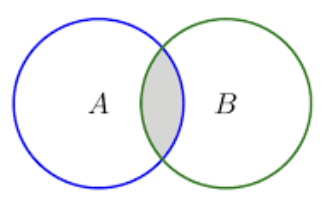
\includegraphics[width=0.3\textwidth]{fig1.png}
\end{center}

\newpage
\begin{mdframed}[
    linewidth=1pt,
    roundcorner=5pt,
    linecolor=ForestGreen,
    innertopmargin=10pt,
    innerbottommargin=10pt
]
{\color{ForestGreen}
\textbf{\underline{Définition :}}}

\vspace{5pt}
L'\textbf{évènement complémentaire} (ou \textbf{évènement contraire}) de $A$ est l'évènement noté $\overline{A}$,
formé de toutes les issues qui ne réalisent pas $A$.

\vspace{5pt}
Autrement dit, $A \cap \overline{A} = \emptyset$ et $A \cup \overline{A} = \Omega$.

\end{mdframed}

\begin{mdframed}[
    linewidth=1pt,
    roundcorner=5pt,
    linecolor=Red,
    innertopmargin=10pt,
    innerbottommargin=0pt
]
{\color{red}
\textbf{\underline{Propriété :}}

\vspace{5pt}
Pour tout évènement $A$, on a :
\[
P(\overline{A}) = 1 - P(A)
\]
}
\end{mdframed}

\begin{mdframed}[
    linewidth=1pt,
    roundcorner=5pt,
    linecolor=RoyalBlue,
    innertopmargin=10pt,
    innerbottommargin=10pt
]
{\color{RoyalBlue}
\textbf{\underline{Exercice d'application n°3:} Calculer la probabilité d'une réunion}}

\vspace{5pt}
On lance un dé à six faces et on considère les événements suivants :

$A$ : « On obtient un nombre impair »

$B$ : « On obtient un multiple de 3 »

\vspace{5pt}
\hspace{0.5cm} a) Calculer $P(A)$, $P(B)$, $P(A \cap B)$.

\hspace{0.5cm} b) Calculer la probabilité de l’événement $A \cup B$. Interpréter le résultat.

\vspace{0.5cm}
{\color{black!30}\dotfill}

\vspace{0.5cm}
{\color{black!30}\dotfill}

\vspace{0.5cm}
{\color{black!30}\dotfill}

\vspace{0.5cm}
{\color{black!30}\dotfill}

\vspace{0.5cm}
{\color{black!30}\dotfill}

\vspace{0.5cm}
{\color{black!30}\dotfill}

\vspace{0.5cm}
{\color{black!30}\dotfill}

\vspace{0.5cm}
{\color{black!30}\dotfill}

\vspace{20pt}

\end{mdframed}

\subsection*{\hspace{1cm} 2) Loi de probabilité}

\vspace{5pt}
\begin{mdframed}[
    linewidth=1pt,
    roundcorner=5pt,
    linecolor=ForestGreen,
    innertopmargin=10pt,
    innerbottommargin=10pt
]
{\color{ForestGreen}
\textbf{\underline{Définition :}}}

\vspace{5pt}
Définir une \textbf{loi de probabilité} pour une expérience aléatoire consiste à attribuer à chacune des issues 
une probabilité.

\end{mdframed}

\vspace{5pt}
\underline{Exemple :}

\vspace{5pt}
Une urne contient 6 boules vertes, 3 boules jaunes et 11 boules noires.

On tire au hasard une boule et on note sa couleur.

Le tableau suivant présente les probabilités de toutes les issues de l'expérience, on l'appelle \textbf{loi de probabilité}.

\vspace{10pt}
% ========================================================
%             % COMMENT FAIRE UN TABLEAU !!!!!
% ========================================================
\begin{tabular}{|>{\centering\arraybackslash}m{3cm}|>{\centering\arraybackslash}m{4cm}|>{\centering\arraybackslash}m{4cm}|
    >{\centering\arraybackslash}m{4cm}|}
    \hline
    \parbox[c][1cm][c]{3cm}{\centering \textbf{Issues}} & 
    \parbox[c][1cm][c]{3cm}{\centering \textbf{Boule verte}} & 
    \parbox[c][1cm][c]{3cm}{\centering \textbf{Boule jaune}} &
    \parbox[c][1cm][c]{3cm}{\centering \textbf{Boule noire}} \\
    \hline
    \parbox[c][2cm][c]{3cm}{\centering \textbf{Probabilités}} & 
    \parbox[c][2cm][c]{4cm}{\centering } 
    & & \\
    \hline
\end{tabular}

\vspace{10pt}
\begin{mdframed}[
    linewidth=1pt,
    roundcorner=5pt,
    linecolor=Red,
    innertopmargin=10pt,
    innerbottommargin=10pt
]
{\color{red}
\textbf{\underline{Propriété :}}
La somme des probabilités de toutes les issues est égale à 1.
}
\end{mdframed}

\begin{mdframed}[
    linewidth=1pt,
    roundcorner=5pt,
    linecolor=RoyalBlue,
    innertopmargin=10pt,
    innerbottommargin=10pt
]
{\color{RoyalBlue}
\textbf{\underline{Exercice d'application n°4:} Utiliser une loi de probabilité}}

\vspace{5pt}
On tire au hasard un jeton dans le sac contenant des jetons numérotés de 1 à 5.
Le tableau présente les probabilités de toutes les issues (loi de probabilité).

\begin{center}
    \begin{tabular}{|>{\centering\arraybackslash}m{3cm}|>{\centering\arraybackslash}m{2cm}|>{\centering\arraybackslash}m{2cm}|
        >{\centering\arraybackslash}m{2cm}|>{\centering\arraybackslash}m{2cm}|>{\centering\arraybackslash}m{2cm}|}
        \hline
        \parbox[c][1cm][c]{2cm}{\centering \textbf{Issues}} & 
        \parbox[c][1cm][c]{2cm}{\centering \textbf{1}} & 
        \parbox[c][1cm][c]{2cm}{\centering \textbf{2}} &
        \parbox[c][1cm][c]{2cm}{\centering \textbf{3}} &
        \parbox[c][1cm][c]{2cm}{\centering \textbf{4}} &
        \parbox[c][1cm][c]{2cm}{\centering \textbf{5}} \\
        \hline
        \parbox[c][2cm][c]{3cm}{\centering \textbf{Probabilités}} & 
        \parbox[c][2cm][c]{2cm}{\centering $\dfrac{1}{15}$} &
        \parbox[c][2cm][c]{2cm}{\centering $\dfrac{4}{15}$} &
        \parbox[c][2cm][c]{2cm}{\centering } &
        \parbox[c][2cm][c]{2cm}{\centering $\dfrac{3}{15}$} &
        \parbox[c][2cm][c]{2cm}{\centering $\dfrac{4}{15}$} \\
        \hline
    \end{tabular}
\end{center}

\hspace{1cm}a) Compléter le tableau de la loi de probabilité.

\hspace{1cm}b) Calculer la probabilité de l’évènement $E$ : « Tirer un chiffre pair ».

\hspace{1cm}c) Décrire l’évènement $\overline{E}$ puis calculer sa probabilité. 

\vspace{0.5cm}
{\color{black!30}\dotfill}

\vspace{0.5cm}
{\color{black!30}\dotfill}

\vspace{0.5cm}
{\color{black!30}\dotfill}

\vspace{0.5cm}
{\color{black!30}\dotfill}

\vspace{0.5cm}
{\color{black!30}\dotfill}

\vspace{0.5cm}
{\color{black!30}\dotfill}


\vspace{20pt}


\end{mdframed}


\section*{\textcolor{red}{Partie 3 : Arbre de probabilités}}

\vspace{5pt}
{\color{ForestGreen}\underline{\textbf{Exemple  définition :}}}

\begin{minipage}[t]{.5\textwidth}%
    \vspace{0pt}
    Dans un sac, on dépose quatre jetons :
    Un bleu, un rouge, un jaune et un vert.

    \vspace{5pt}
    On tire un jeton, on note sa couleur et on le remet dans le sac.
    On retire un jeton et on note à nouveau sa couleur.

    \vspace{5pt}
    À chaque tirage, on a 4 issues possibles.

    On représente l'ensemble de l'expérience par un arbre.

    \vspace{10pt}
    \textbf{1) Calculer la probabilité d'obtenir un jeton vert et un jeton bleu (l'ordre de 
    compte pas).}

    \vspace{0.5cm}
    {\color{black!30}\dotfill}
    
    \vspace{0.5cm}
    {\color{black!30}\dotfill}

\end{minipage}%
\hfill
\begin{minipage}[t]{.45\textwidth}%
    \vspace{-20pt}
    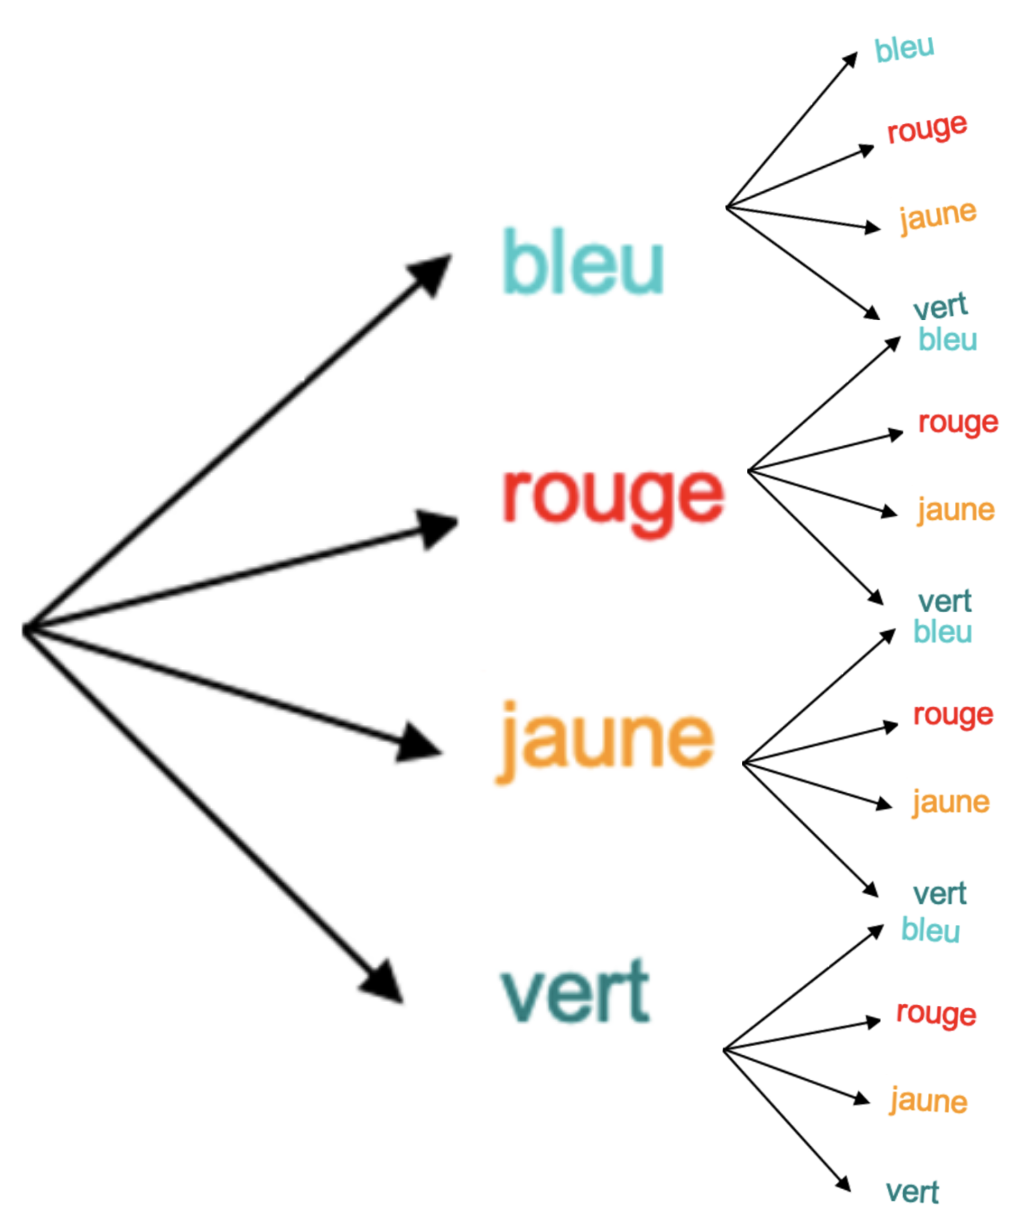
\includegraphics[width=1\textwidth]{fig2.png}
\end{minipage}%

\vspace{10pt}
\textbf{2) Calculer la probabilité d'obtenir 2 jetons rouges.}

\vspace{0.5cm}
{\color{black!30}\dotfill}

\vspace{0.5cm}
{\color{black!30}\dotfill}

\vspace{0.5cm}
{\color{black!30}\dotfill}

\begin{mdframed}[
    linewidth=1pt,
    roundcorner=5pt,
    linecolor=RoyalBlue,
    innertopmargin=10pt,
    innerbottommargin=10pt
]
{\color{RoyalBlue}
\textbf{\underline{Exercice d'application n°5:} Utiliser un arbre de probabilités}}

\vspace{5pt}
On lance deux fois de suite une pièce de monnaie. Il s’agit d’une expérience aléatoire à deux
épreuves.

\vspace{5pt}
Soit $E$ l’événement : « On obtient au moins une fois PILE. »

\vspace{5pt}
Calculer $P(E)$ en utilisant un arbre des possibles.

\begin{minipage}[t]{.5\textwidth}%
    \vspace{0pt}
    \vspace{0.5cm}
    {\color{black!30}\dotfill}

    \vspace{0.5cm}
    {\color{black!30}\dotfill}

    \vspace{0.5cm}
    {\color{black!30}\dotfill}

    \vspace{0.5cm}
    {\color{black!30}\dotfill}

    \vspace{40pt}
\end{minipage}%
\hfill
\begin{minipage}[t]{.45\textwidth}%
    \vspace{0pt}
    
\end{minipage}%


\end{mdframed}







\end{document}
